%%%%%%%%%%%%%%%%%%%%%%%%%%%%%%%%%%%%%%%%%%%%%%%%%%%%%%%%%%%%%%%%%%%%%%%%%%%%%%%%
\documentclass[twocolumn]{revtex4}

%%%%%%%%%%%%%%%%%%%%%%%%%%%%%%%%%%%%%%%%%%%%%%%%%%%%%%%%%%%%%%%%%%%%%%%%%%%%%%%%
% Note that comments begin with a "%" and are not turned into text in the .pdf
% document.
%%%%%%%%%%%%%%%%%%%%%%%%%%%%%%%%%%%%%%%%%%%%%%%%%%%%%%%%%%%%%%%%%%%%%%%%%%%%%%%%

%%%%%%%%%%%%%%%%%%%%%%%%%%%%%%%%%%%%%%%%%%%%%%%%%%%%%%%%%%%%%%%%%%%%%%%%%%%%%%%%
% Include some extra packages.
%%%%%%%%%%%%%%%%%%%%%%%%%%%%%%%%%%%%%%%%%%%%%%%%%%%%%%%%%%%%%%%%%%%%%%%%%%%%%%%%
\usepackage[]{graphicx}
%%%%%%%%%%%%%%%%%%%%%%%%%%%%%%%%%%%%%%%%%%%%%%%%%%%%%%%%%%%%%%%%%%%%%%%%%%%%%%%%

%%%%%%%%%%%%%%%%%%%%%%%%%%%%%%%%%%%%%%%%%%%%%%%%%%%%%%%%%%%%%%%%%%%%%%%%%%%%%%%%
\begin{document}

%%%%%%%%%%%%%%%%%%%%%%%%%%%%%%%%%%%%%%%%%%%%%%%%%%%%%%%%%%%%%%%%%%%%%%%%%%%%%%%%
\title{
Final Project: Can you escape a Velociraptor?
}

\author{S. Caruso}
\affiliation{Siena College, Loudonville, NY}

\date{\today}

\begin{abstract}
    
    To figure out if I can escape a velociraptor, I had to perform four tasks using Python code.  To do this, I used a series of while loops, graphs, and one function.  The first task was to plot position vs. time.  The second task was  to figure out when the raptor catches up to the human.  Results were in two seconds when the human had run 6 meters.  The third task was to figure out when the raptor would be one meter behind the human.  The results were that 1.933334 seconds had passed and the human had run 5.800002 meters.  For this task, I also had to add an arrow to the previous graph pointing to the point at which the velociraptor was one meter away from the human.  The last task was to see if the velociraptor would bite the human.  The results were that there is about a 60 percent chance the human will get away. 
\end{abstract}


%%%%%%%%%%%%%%%%%%%%%%%%%%%%%%%%%%%%%%%%%%%%%%%%%%%%%%%%%%%%%%%%%%%%%%%%%%%%%%%%
\maketitle
%%%%%%%%%%%%%%%%%%%%%%%%%%%%%%%%%%%%%%%%%%%%%%%%%%%%%%%%%%%%%%%%%%%%%%%%%%%%%%%%
\section{Introduction}
	Have you ever thought to yourself: "Self, will I ever get chased by a velociraptor? If I find myself in this situation, when will he catch me and what are my chances of getting away?"  Look no further, because this write-up will answer all questions you will ever need answered. In this scientific paper, I will provide graphs, and proven evidence that provides you with the information you NEED for your velociraptor concerns.
%%%%%%%%%%%%%%%%%%%%%%%%%%%%%%%%%%%%%%%%%%%%%%%%%%%%%%%%%%%%%%%%%%%%%%%%%%%%%%%%


%%%%%%%%%%%%%%%%%%%%%%%%%%%%%%%%%%%%%%%%%%%%%%%%%%%%%%%%%%%%%%%%%%%%%%%%%%%%%%%%
\section{Problem 1:Position vs. time}
	For problem 1: position vs. time, I first imported matplotlib as plt to allow me to plot a graph.  I then made a varianle called t that represents the linspace of the plot.  The linspace goes from zero to two.  The variable v represents the position which a velociraptor is at any given point in time.  The variable h represents the position which a human is at any given point in time.  The equations for these two variables can be found at the end of the paper.  I then make two errorbars, one plotting the velociraptor's position and the other plotting the human's position.  I label the x-axis 'Time' and the y-axis 'Position.'  I title the graph 'Human vs. Velociraptor' and make a legend stating which points represent the human's positions and which points represent the velociraptor's position.  Lastly, I make the legend's position '4' to place it in the bottom right of the graph. The graph can be found in the last section of the paper.

\section{Problem 2:When does the 'raptor catch up to you?}	
	For problem 2: when does the 'raptor catch up to you? I first set variable ph to 30.  This represents the starting position of the human.  I then set both pv and time to 0, representing the starting position of the velociraptor and the starting time.  After this, I made a while loop so that whenever the human's position is not equal to the velociraptor's position, I add 3 to the human's position, 18 to the velociraptor's position and increment time.  I do this because we are given that a human runs 3 m/s and a velociraptor runs 18 m/s.  When the human's position is equal to the velociraptor's position, I print time and the distance the human ran which is the human's position minus 30.
\section{Problem 3:When is it close enough to strike?}
For problem 3: when is it close enough to strike, I make another while loop so that whenever the human's position minus the velociraptor's position is greater than 1, I add .000003 to the human's position, .000018 to the velociraptor's position, and .00001 to time.  I do this because we are given the human's and velociraptor's speeds.  Instead of incrementing time, I add .000001 to make the algorithm loop more, ultimately giving a more accurate representation.  After the while loop, I print how many seconds had passed and how far the human ran.  Following this print statement, I make a graph that includes an arrow pointing to the point at which the velociraptor is 1 meter away from the human.  I do this by using the same code from the last graph and adding an annotate command.  This command adds the arrow which points to the x,y point, (time,velociraptor position.)	  The graph can be found in the last section of this paper.
\section{Problem 4: Will it bite you?}
For problem 4: will it bite you, I first import numpy to generate random numbers for later on.  I then make a function called probability that takes in no variables.  The function produces three variables, x, y, and z, which are three different random numbers from 0 to 100.  Within the function, I make an if statement which says that if x is between 1 and 20, the function returns a string that says "You're raptor food."  If not, the function goes into into an elif which says that is y is between 1 and 15, the function returns a string that says "You're raptor food."  If not, the function goes into another elif saying that if z is between 1 and 7, the function returns a string that says "You're raptor food."  If not, the function returns a string that says "You get away!"  I do this because the 'raptor takes three bites at the human.  The first bite has a 20 percent chance of hitting, the second bite has a 15 percent chance of hitting, and the third bite has a 7 percent chance of hitting.  If none of these hit, the human gets away.  To calculate the probability, I set three variables, n, raptorwin, and humanwin, to 0.  I then run 1000 trials using a while loop.  The loop says that if n is less than 1000, I run the probability function.  If the function returns "You're raptor food," I increment the variable raptorwin.  If the function returns "You get away." I increment humanwin.  After this, I increment n.  Lastly, I make a variable p that is humanwin/1000.  This will represent an approximation of the probability of the human getting away from the velociraptor.      
\section{Graphs and Equations}
\begin{figure}[h!]
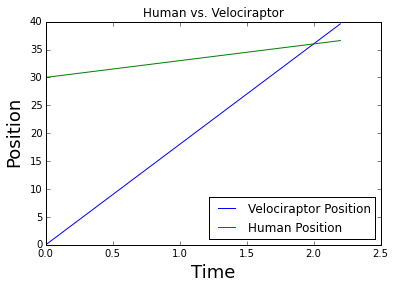
\includegraphics[width=\linewidth]{goodplot1.png}
\caption{Graph comparing the positions of the human and the velociraptor.}
\end{figure}
\begin{figure}[h!]
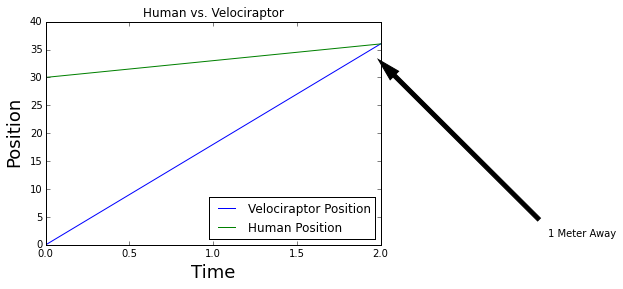
\includegraphics[width=\linewidth]{goodplot2.png}
\caption{Graph with arrow pointing to when the velociraptor is 1 meter away from the human.}
\end{figure}


Equation used to find position: $$p = v*t + p_0$$

%%%%%%%%%%%%%%%%%%%%%%%%%%%%%%%%%%%%%%%%%%%%%%%%%%%%%%%%%%%%%%%%%%%%%%%%%%%%%%%%

%%%%%%%%%%%%%%%%%%%%%%%%%%%%%%%%%%%%%%%%%%%%%%%%%%%%%%%%%%%%%%%%%%%%%%%%%%%%%%%%
\end{document}
%%%%%%%%%%%%%%%%%%%%%%%%%%%%%%%%%%%%%%%%%%%%%%%%%%%%%%%%%%%%%%%%%%%%%%%%%%%%%%%%
